\documentclass{article}
\usepackage[utf8]{inputenc}
\usepackage[english]{babel}
\usepackage{fullpage}
\usepackage[top=4cm, bottom=4cm, left=4cm, right=4cm]{geometry} 
\usepackage{amsmath,amsthm,amsfonts,amssymb,amscd}
\usepackage{lastpage}
\usepackage{mathtools}
\usepackage{enumerate}
\usepackage{fancyhdr}
\usepackage{mathrsfs}
\usepackage{xcolor}
\usepackage{graphicx}
\usepackage{listings}
\usepackage{hyperref}
\usepackage{setspace}
\usepackage{mathtools}
\usepackage{dirtytalk}
\usepackage{mathrsfs}
\usepackage{tikz}
\usepackage{tkz-euclide}
\usepackage{tikz-cd}
\usepackage{wrapfig}

\newtheorem{theorem}{Theorem}[section]
\newtheorem{lemma}{Lemma}[section]
\newtheorem{proposition}{Proposition}[section]
\newtheorem{remark}{Remark}[section]
\newtheorem{definition}{Definition}[section]
\newtheorem{corollary}{Corollary}[section]
\newtheorem{example}{Example}[section]
\newtheorem{conjecture}{Conjecture}[section]

\title{Classifying Brieskorn Varieties and Brieskorn Manifolds}
\author{Thomas Sachen\\[1ex] 
\small Chenyang Xu (Advisor)}
\date{April 2022}

\doublespacing

\begin{document}

\maketitle

\begin{abstract}
    This paper is an exposition of several results classifying \textit{Brieskorn varieties,} complex algebraic varieties that arise as the vanishing loci of polynomials of the form $z_1^{a_1} + \dots + z_n^{a_n}$. I survey results of Hamm, Milnor, Neumann, and others from the 1960s and 1970s, concluding with a view toward modern developments, generalizations, and further directions for research.
\end{abstract}

\section{Introduction}

While the study of singularities of algebraic curves dates back to the late nineteenth century and the work of Klein and Brauer, it was given new life in 1961, when David Mumford discovered the following surprising fact: the boundary $K$ of a small neighborhood of a point $p$ in a complex surface is simply connected if and only if the point is smooth and $K$ is homoemorphic to the usual $3$-sphere. The proximity of this result to the classical Poincar\'{e} conjecture (in particular, the implication that one cannot find a counterexample to the Poincar\'{e} conjecture using complex singularities) initiated a period of work by Milnor, Brieskorn, Pham, and others investigating the so-called \say{links} associated to complex singularities, along the way discovering many key results that helped shape the subsequent development of algebraic geometry, algebraic topology, and knot theory.
Milnor's 1967 work \textit{Singular Points of Complex Hypersurfaces} brought this field into the mainstream, introducing several very useful theorems and conjectures that would drive research for the next several decades. Indeed, this work has proved to be invaluable in the study of projective curves and complex geometry.

This paper is a survey of many important results thus far, with a view at the end toward modern techniques and directions for further research. In particular, the focus will be on so-called \textit{Brieskorn manifolds}, a special class of link arising from complex \textit{Brieskorn varieties} of the form $z_1^{a_1} + z_2^{a_2} + \dots + z_n^{a_n},$ with the $a_i$ integers greater than $1$. In the case $n=2$, the link of $0$ for a Brieskorn variety $\{z_1^p + z_2^q = 0\}$ with $p$ and $q$ coprime is a $(p,q)$-torus knot. In particular we'll focus on Milnor's classification of these manifolds up to diffeomorphism in the case $n=3$ \cite{milnor_1975}. Properties for higher $n$ will also be discussed in some detail.

\section{Definitions and Basic Notions}

A \textit{complex algebraic set} $V \subset \mathbb{C}^n$ is the common vanishing locus of a collection of elements of $\mathbb{C}[z_1, \dots z_n].$ Furthermore, an important result of Hilbert (the so-called \say{Hilbert basis theorem}) asserts that any such set is expressible as the vanishing locus of a finite collection of polynomials.[reference] If a non-empty algebraic set $V$ cannot be written as the union of two proper algebraic subsets of $\mathbb{C}^n,$ it is called a \textit{complex algebraic variety} or, for our purposes, simply a \textit{variety}. 

Let $V$ be a variety defined as the vanishing locus of polynomials $f_1, \dots, f_m \in \mathbb{C}[z_1, \dots, z_n]$. We have the following definitions \cite{milnor_1968}.

\begin{definition}

A point $x \in V$ is \textbf{singular} if the Jacobian matrix J with entries $J_{ij} = \partial f_i/\partial z_j$ fails to be injective at $x$, or in other words if $J$ does not attain its maximal rank at $x$. In this case, $x$ is called a \textbf{singular point of V}, or simply a \textbf{singularity}.

\end{definition}
\begin{remark}
Singularities are not dependent on our choice of the $f_i$ defining $V$. If for instance we append a polynomial $f_{m+1} = a_1f_1 + \dots + a_mf_m$ to $\{f_1, \dots, f_m\}$ and define $$V' = \{z \in \mathbb{C}^n\ :\ f_i(z) = 0 \mathrm{\ for\ }i= 1, \dots m+1\}$$ with a corresponding Jacobian $J'$, then the $m+1$\textsuperscript{th} row of $J'$ is a linear combination of the first $m$ rows.
\end{remark}

An important note at this point is the smooth manifold structure of real and complex algebraic varieties away from singularities. Letting $\Sigma(V)$ denote the set of singularities of a complex algebraic set $V \subset \mathbb{C}^n$, then $V \setminus \Sigma(V)$ is a smooth complex analytic manifold. This is also true in the real setting after appropriate modifications, and the reader is referred to \cite{whitney_1957} for proof and a more detailed treatment.

We will also need to define the \textit{link} of a point $p \in V$. Informally, the link $K$ of $p$ is the intersection $K= S_{\epsilon} \cap V$, where $S_{\epsilon}$ is a small sphere of radius $\epsilon$ centered at $p$. In order to make this definition precise, however, we must be careful with our choice of $\epsilon$ to ensure that $V$ intersects $S_\epsilon$ transversally. That such an $\epsilon$ exists is not entirely obvious. We also must be careful that a particular choice of $\epsilon$ does not affect the topology of $K$. 

These concerns are addressed in the following results of Milnor\cite{milnor_1968}. Let $V$ be a complex variety with an isolated singularity (or smooth point) $p$. Let $S_\epsilon$ (resp. $D_{\epsilon}$) denote the small sphere (resp. closed disk) of radius $\epsilon$ centered at $p$.
\begin{proposition}
For every sufficiently small $\epsilon$, $S_\epsilon$ intersects $V$ in a smooth (possibly vacuous manifold). Furthermore, the intersection is transverse, in the sense that any element of the tangent space of a point of $V \cap S_\epsilon$ may be written as the sum of a tangent vector to $V$ and a tangent vector to $S_{\epsilon}.$
\end{proposition}
\begin{proposition}
\label{2.2}
For sufficiently small $\epsilon$ the intersection of $V \cap D_{\epsilon}$ is homeomorphic to the cone over $K = V \cap S_{\epsilon}.$ In fact, we have the following homeomorphism of pairs:
\[(D_{\epsilon}, V \cap D_{\epsilon}) \simeq \mathrm{Cone}(S_{\epsilon}, S_{\epsilon} \cap V),\]
where $S_{\epsilon} = \partial D_{\epsilon}.$
\end{proposition}

Elegant proofs of these facts can be found in \cite{milnor_1968}. The upshot of this discussion is that the link $K$ of a point is topologically well-defined (up to diffeomorphism) with respect to shrinking $\epsilon,$ provided that $\epsilon$ is chosen to be sufficiently small as to satisfy propositions 2.1 and 2.2. We are therefore able to make the following definition, with terminology as in the above propositions.
\begin{definition}
The \textbf{link} $K$ of a point $p \in V$ is the smooth manifold given by $K = V \cap S_{\epsilon},$ for $\epsilon$ sufficiently small.
\end{definition}

\section{Brieskorn Varieties}

An interesting example of complex variety, the analysis of which will form the heart of this paper, is a \textit{Brieskorn variety:}
\begin{definition}
A \textbf{Brieskorn variety} $V_{(a_1, \dots, a_n)}$ is an algebraic variety defined as the vanishing locus of the polynomial
\[z_1^{a_1} + z_2^{a_2} + \dots + z_n^{a_n},\]
with each $a_i$ an integer greater than $1$.
\end{definition}
It is easily checked that a Brieskorn variety has a unique singularity at the origin. This motivates the following definition:
\begin{definition}
The \textit{Brieskorn manifold} $K_{(a_1, \dots, a_n)}$ is the link of the origin with respect to the Brieskorn variety $V_{(a_1, \dots, a_n)}$. That is, 
\[K_{(a_1, \dots, a_n)} = V_{(a_1, \dots, a_n)} \cap S_\epsilon,\]
for sufficiently small $\epsilon.$
\end{definition}

We will usually simply refer to a Brieskorn variety as $V$ and the associated Brieskorn manifold as $K,$ provided the $a_i$ are clear from context.

A suggestive example of why Brieskorn manifolds are of particular interest is in the case $n=2.$ First recall that a \textit{torus knot} $T$ is a simple closed curve that lies on the surface of an unknotted torus $\mathbb{T}$. Each such knot is determined up to ambient isotopy by a pair of coprime integers $(p,q)$, where $p$ specifies the number of times $T$ wraps around $\mathbb{T}$ meridianally, and $q$ the number of times $T$ wraps around $\mathbb{T}$ longitudinally. A torus knot specified by such $p$ and $q$ is called a \textit{torus knot of type $(p,q)$} or a \textit{(p,q)}-torus knot, and is denoted here by $T_{(p,q)}$. Note in particular that $T_{p,q}$ is ambient isotopic to $T_{q,p}$.

Returning to the case of Brieskorn manifolds, we have the following proposition, owing to Brauner in 1928 \cite{brauner_1928}. Let $p$ and $q$ be coprime positive integers. Then
\begin{proposition}
The Brieskorn manifold $K_{(p,q)}$ is a torus knot of type $(p,q)$.
\end{proposition}
\begin{proof}
First note that an unknotted torus $\mathbb{T} \subset \mathbb{C}^2$ can be specified by 
\[\mathbb{T}_c = \{(z_1, z_2) \in \mathbb{C}^2\ :\ |z_1| = |z_2| = c\},\]
for $c$ a positive real constant. Indeed, we can write $K$ up to isotopy as $K = \{z_1^p = z_2^q\} \cap \{|z_1|^2 = |z_2|^2 = 2\}$, so $K \subset \mathbb{T}_1,$ and in particular $K$ is the set of points $(z_1, z_2)$ satisfying $p \cdot \mathrm{arg}z_1 = q \cdot \mathrm{arg}z_2$. Hence we may parametrize $K$ as the path $[0, 2pq \pi] \to K$ via the assignment $t \mapsto (e^{it/p}, e^{it/q})$. In doing so we ensure that the first coordinate wraps around the torus $q$ times longitudinally and the second coordinate wraps around the torus $p$ times meridianally, so indeed $K$ is a $(p,q)$-torus knot.

\end{proof}

This is an interesting fact, but it does not reveal much in the way of rich topological or analytic structure. For this, we turn to the work of Brieskorn and generalizations in higher dimensions. To motivate this study and indeed to view Brieskorn manifolds as, in some sense, a natural generalization of torus knots, we have the following \cite{milnor_1975}

\begin{proposition}
The Brieskorn manifold $K_{(a_1, a_2, a_3)}$ is homeomorphic to the $a_3$-fold cyclic branch covering of $S^3,$ with branch locus $T_{a_1, a_2}.$
\end{proposition}
\begin{proof}
Writing $V = \{ z_1^{a_1} + z_2^{a_2} + z_3^{a_3} = 0\}$, consider the projection map $\pi:V \setminus \{0\} \to \mathbb{C}^2 \setminus \{0\}$ given by $(z_1, z_2, z_3) \mapsto (z_1, z_2)$. Then clearly $\deg(\pi) = a_3,$ and furthermore we may cyclically permute the $a_3$ preimages via the action of $\Omega$, the group of $a_3$\textsuperscript{th} roots of unity. For any $\omega \in \Omega,$ the action is given explicitly by $\omega \cdot (z_1, z_2, z_3) = (z_1, z_2, \omega z_3).$ In particular there is a homeomorphism $(V\setminus \{0\} )/\Omega \xrightarrow{\sim} \mathbb{C}^2 \setminus \{0\},$ from which we may conclude that $V\setminus\{0\}$ is an $a_3$-fold cyclic branched covering of $\mathbb{C}^2 \setminus \{0\}$ branched along $\{z_1^{a_1} + z_2^{a_2} = 0\}.$

Now consider the action of $\mathbb{R}^+$ on $V \setminus \{0\}$ given by \[t \cdot (z_1, z_2, z_3) = (t^{a_1^{-1}}z_1, t^{a_2^{-1}}z_2, t^{a_3^{-1}}z_3)\] for $t \in \mathbb{R}^+.$ Noticing that the $\mathbb{R}^+$-orbit of any $z \in V$ under this action (transversally) intersects the unit sphere precisely once, there is a canonical diffeomorphism $V \setminus \{0\} \simeq \mathbb{R}^+ \times K_{(a_1, a_2, a_3)}$. 

In a similar vein there is an action of $\mathbb{R}^+$ on $\mathbb{C}^2 \setminus \{0\}$ given by \[t \dot (z_1, z_2) = (t^{a_1^{-1}}z_1, t^{a_2^{-1}}z_2),\] inducing a canonical diffeomorphism $\mathbb{C}^2 \setminus \{0\} \simeq \mathbb{R}^3 \times S^3.$ Finally, observing that the $\mathbb{R}^+$ action and $\Omega$ action on $V \setminus \{0\}$ commute, as well as the fact that $\pi$ is $\mathbb{R}^+$-equivariant, we may conclude that $K_{(a_1, a_2, a_3)}$ is an $a_3$-fold cyclic branched covering of $S^3$, branched over $T_{a_1, a_2}.$

\end{proof}

\section{Classifying Brieskorn 3-manifolds}

Proposition 3.2. gives a useful topological description of Brieskorn manifolds with $3$ parameters, but we can also view them more geometrically. This section is devoted to studying Milnor's description of these manifolds \cite{milnor_1975}. We study his constructions in some detail, in order to build a foundation of the basic theory, before moving to further results and more recent develops in \S 5. To do so we first recall some notions from classical plane geometry.

There has been much work done on the classical \textit{triangle groups}, a keystone of the geometry of the late 19\textsuperscript{th} and early 20\textsuperscript{th} centuries. While there is a very beautiful theory around these objects (cf. [references]), we'll only build up the facts necessary for our purposes. Let $P$ be either the Euclidean plane, the hyperbolic plane, or the sphere with the usual metric.
\begin{definition}
A \textbf{full triangle group} $\overline{\Delta}(p,q,r)$ is a group of reflections of $P$ specified by positive integers $p,q,r$, with presentation
\[\overline{\Delta}\langle a,b,c\ |\ a^2 = b^2 = c^2 = (ab)^p = (bc)^r = (ca)^q = 1\rangle.\]
The corresponding \textbf{triangle group} $\Gamma(p,q,r) \leq \overline{\Delta}(p,q,r)$ is the index two subgroup of words of even length, which correspond to orientation preserving transformations of $P$.
\end{definition}
The role of $(p,q,r)$ in determining the reflection action of $\overline{\Delta}$ on $P$ is as follows. For a fixed full triangle group $\overline{\Delta}(p,q,r),$ the fundamental domain for the action of $\overline{\Delta}(p,q,r)$ on $P$ is a triangle $\Delta$ with interior angles $\pi/p, \pi/r, \pi/q$ (Figure 1).
\begin{figure}
    \centering
    \includegraphics[scale=.45]{images/triangle.png}
    \caption{A fundamental domain for the action of the full triangle group $\overline{\Delta}(p,q,r).$}
\end{figure}
This action is given by reflecting over each the edges of $\Delta$, noting that the composition of reflections over two adjacent edges is the same as a rotation by twice the angle between those edges. The geometry of $P$ is determined according to whether
\begin{enumerate}[(i)]
    \item $\frac{1}{p} + \frac{1}{q} + \frac{1}{r} = 1$, where $P$ is Euclidean;
    \item $\frac{1}{p} + \frac{1}{q} + \frac{1}{r} < 1$, where $P$ is hyperbolic; or
    \item $\frac{1}{p} + \frac{1}{q} + \frac{1}{r} > 1$, where $P$ is spherical,
\end{enumerate}
by the Gauss-Bonnet theorem. The orbit of the fundamental domain triangle, of course, gives a tiling of $P$, the tiles of which are pairwise disjoint except for shared edges.

\subsection{The spherical case}

This subsection will give a description of the Brieskorn manifolds $K_{(p,q,r)}$ for which $\frac{1}{p} + \frac{1}{q} + \frac{1}{r} > 1$. A classical result is that the Lie group $S^3$ with quaternionic group structure is a double covering of $\mathrm{SO(3)}$, the rotation group of $S^2$ via the projection $\pi: S^3 \to \mathrm{SO}(3),$ with $\ker \pi = \{\pm 1\} = Z(S^3)$ (this is Dirac's \say{belt trick}). Note also that $S^3 \simeq \mathrm{SU}(2)$, the group of special unitary $2\times 2$ matrices. We also have the following famous theorem, given here without proof, but for which a more detailed treatment can be found in \cite{artin_2011}. In the spherical case,
\begin{theorem}
\label{4.2}
Any finite subgroup of $\mathrm{SO}(3)$ is one of the following, for an integer $k$:
\begin{enumerate}[(i)]
    \item $C_k$, the cyclic group of rotations by multiples of $2 \pi/k$ about a line;
    \item the dihedral group $D_k$ of symmetries of a regular $k$-gon, isomorphic to $\Delta(2,2,k)$;
    \item the tetrahedral group $T$ of $12$ rotational symmetries of a tetrahedron, isomorphic to $\Delta(2,3,3)$;
    \item the octahedral group $O$ of $24$ rotational symmetries of an octahedron, isomorphic to $\Delta(2,3,4)$; or
    \item the icosahedral group $I$ of $60$ rotational symmetries of an icosahedron, isomorphic to $\Delta(2,3,5).$
\end{enumerate}
\end{theorem}
Therefore, an order $n$ subgroup of $\mathrm{SO}(3)$ lifts to an order $2n$ subgroup of $S^3$. These are the so-called \textit{binary polyhedral groups} of order $2k, 4k, 24, 48,$ and $120$ in comparison with the list above. We denote such a lifting of a triangle group $\Delta(p,q,r)$ by $\Gamma(p,q,r)$. With this in mind, we may prove the following proposition \cite{seade_2006}.
\begin{proposition}
The only finite subgroups of $S^3$ are the double covers of the finite subgroups of $\mathrm{SO}(3)$, and cyclic subgroups of odd order.
\end{proposition}
\begin{proof}
Let $H$ be an arbitrary finite subgroup of $S^3 \simeq \mathrm{SU}(2)$. If $H$ contains the center $\{\pm 1\} = Z(\mathrm{SU}(2)),$ then it is the lift of a finite subgroup of $\mathrm{SO}(3),$ by definition of the projection map $\pi.$ Hence we may assume that $H$ does not contain $\pm 1$. Let $g \in \mathrm{SU}(2)$ be an element of order $2$, of the form
\[g = \begin{pmatrix} z_1 & z_2\\ -\overline{z}_2 & \overline{z}_1\end{pmatrix}\]
with $|z_1|^2 + |z_2|^2 = 1$ and $g^2 =1$. Then $z_1$ and $z_2$ must satisfy $z_2(z_1 + \overline{z}_1) = \overline{z}_2(z_1 + \overline{z}_1) = 0,$ so either $z_2 = 0$ or $z_1$ is pure imaginary. But the latter is impossible: writing $z_1 = ti$ for some $t \in \mathbb{R},$ then $z_1^2 = -t^2 \leq 0,$ but by the requirement $g^2 = 1$ we must also have that $z_1^2 - |z_2|^2 = 1,$ a contradiction. Therefore we must have $z_2 = 0$ and $z_1 = \pm 1$.

Since all elements of $H$ except possibly $1$ come in pairs with their inverses, if $-1 \not\in H$ then $|H|$ is odd. Finally, since $H$ does not contain $\{\pm 1\} = \ker \pi$ the restricted projection $\pi|_{H}$ is injective, hence $H$ is isomorphic to its image $\pi(H).$ Therefore $H$ is isomorphic to a subgroup of $\mathrm{SO}(3)$ of odd order, which must be cyclic by Theorem \ref{4.2}.

\end{proof}

Of course, $\mathrm{SU}(2)$ acts linearly on $\mathbb{C}^2$ by matrix multiplication. Since elements of $\mathrm{SU}(2)$ are unitary, this action fixes the origin, but is free everywhere else in $\mathbb{C}^2$ and it is stable on all spheres centered at the origin. In particular, there is an induced action of any finite subgroup $\Gamma \leq \mathrm{SU}(2)$ on $\mathbb{C}^2$. The space $\mathbb{C}^2/\Gamma$ of orbits of this action is a complex variety I'll denote by $V_{\Gamma},$ which has a unique singularity at the origin \cite{hirzebruch_1987}. Then the link of the origin (with $\epsilon=1$) is the orbit space $K = \Gamma/S^3$, a smooth $3$-manifold with universal cover $S^3$ and $\pi_1(K) = \Gamma$.

 Let $V^d$ denote the vector space of degree $d$ homogeneous polynomials in two complex variables $z_1$ and $z_2$. It's easy to show that $\dim V^d = d+1,$ with basis $$\{z_1^d, z_1^{d-1}z_2, \dots, z_1z_2^{d-1}, z_2^d\}.$$
 Now, we say a complex polynomial is \textit{$\Gamma$-invariant} if $f(z_1, z_2) = f(\gamma(z_1, z_2))$ for all $\gamma \in \Gamma$ and all $(z_1, z_2) \in \mathbb{C}^2$. Let $V^n_\Gamma$ denote the subspace of $V^n$ consisting of the $\Gamma$-invariant degree $d$ homogeneous polynomials. Indeed, since the product of an element of $V_\Gamma^{d_1}$ and an element of $V_\Gamma^{d_2}$ is an element of $V_\Gamma^{d_1 + d_2},$ we have that
 \[V^*_\Gamma = \bigoplus_{q = 0}^\infty V^q_\Gamma\]
 is an $\mathbb{N}$-graded algebra with respect to polynomial multiplication. Now we can give a description of these Brieskorn manifolds in the spherical case, due to Milnor \cite{milnor_1975}.
 \begin{theorem}
 \label{Theorem 4.2}
 Let $p,q,r$ such that $p^{-1} + q^{-1} + r^{-1} > 1$. Let $\Gamma(p,q,r) = \Gamma$ be a binary triangle subgroup of $\mathrm{SU}(2)$ with commutator subgroup $\Pi = [\Gamma, \Gamma]$. Then $V^*_\Gamma$ is generated by three polynomials $f_1, f_2, f_3$ of order $k/p, k/q, k/r$ respectively, where $k$ is the order of $\Gamma$ inside $\mathrm{SU}(2).$ Furthermore, the $f_i$ satisfy the single\footnote{This is shorthand, to say that the ideal of all relations among the $f_i$ is generated by this single relation.} relation
 \[f_1^p + f_2^q + f_3^r = 0.\]
Moreover, the map from $\mathbb{C}^2$ to $\mathbb{C}^3$ given by $z \mapsto (f_1(z), f_2(z), f_3(z))$ maps the orbit space $\mathbb{C}^2/\Pi$ homeomorphically to $V_{(p,q,r)}.$ This map is actually a diffeomorphism away from the origin, and in particular it induces a diffeomorphism between the corresponding links $\mathrm{SU(2)}/\Pi$ and $K_{(p,q,r)}.$
 \end{theorem}
 We will go through the proof of this theorem in some detail, as structurally it's very similar to the hyperbolic case. We first prove several lemmas Let $\chi$ be a character of $\Gamma,$ \textit{i.e.} a one-dimensional unitary representation $\chi: \Gamma \to U(1) \simeq \mathbb{C}\setminus \{0\}.$ Let $V^{d, \chi}_\Gamma$ denote the space of $d$-homogeneous polynomials $f$ such that
 \[f(\gamma(z)) = \chi(\gamma)f(z)\]
 for all $\gamma \in \Gamma$ and $z \in \mathbb{C}^2$.  Notice that, by definition, $V^{\ast,1}_\Gamma = V_\Gamma^\ast.$ Noting that for $f \in V_\Gamma^{d_1, \chi_1}$ and $g \in V_\gamma^{d_2, \chi_2},$ $fg \in V_\Gamma^{d_1+d_2, \chi_1\chi_2}$, by taking direct sums we obtain a bigraded algebra which we denote as $V^{\ast, \ast}_\Gamma,$ with an identity element $1$.
 \begin{lemma}
 \label{4.1}
 The space $V_\Pi^{d,1}$ is a direct sum of the subspaces $V_\Gamma^{d,\chi},$ where $\chi$ varies over all characters of $\Gamma$. 
 \end{lemma}
\begin{proof}
 The inclusion $V_\Gamma^{d,\chi} \subset V_\Pi^{d,1}$ is clear, since each character of $\Gamma$ is the trivial map when restricted to $\Pi$. For the other inclusion, first note that the abelianization $\Gamma/\Pi$ acts linearly (on the right) on $V_{\Pi}^{n,1},$ since $\Pi$ is a normal subgroup. For arbitrary $\gamma \in \Gamma$ and $\pi \in \Pi,$ let $f_\gamma$ denote the polynomial $z \mapsto f(\gamma(z))$. Then
 \[(f_\gamma)\pi = (f(\gamma \pi \gamma^{-1}))\gamma = f_\gamma,\]
 using the fact that the quotient group is abelian. Hence we conclude that $f_\gamma$ is actually $\Pi$-invariant. Furthermore, since $f_{\gamma_1} = f_{\gamma_2}$ whenever $\gamma_1$ and $\gamma_2$ differ by an element of $\pi$, and $\Gamma/\Pi$ is finite and abelian, we have an eigenspace decomposition of $V_{\Pi}^{n,1}$ with each eigenspace corresponding to a character of $\Gamma/\Pi$, as desired.
\end{proof}
Now we demonstrate a key correspondence between homogeneous polynomials and characters of $\Gamma$. Let $h \in V^{d, \chi}_\Gamma$ for arbitrary $d$ and $\chi$. Then, by the fundamental theorem of algebra, $h$ vanishes along $d$ lines (with multiplicity) $L_1, \dots, L_d$ through the origin in $\mathbb{C}^2$, which are permuted by any $\gamma \in \Gamma.$ Furthermore, given $d$ lines through the origin in $\mathbb{C}^2$ on which $\Gamma$ acts by permutation, there is associated a unique (up to a scalar multiple) $d$-homogeneous polynomial $f$. Then $f$ has the property that $f(\gamma(z))$ is a scalar multiple of $f(z)$ for any $\gamma,$ so in particular we may define a character $\chi$ via
\[\chi(\gamma) = \frac{f(\gamma(z))}{f(z)},\]
so that $f \in V^{n, \chi}_\Gamma.$ 

Now, consider the natural action of $\mathrm{SU}(2)$ on $\mathbb{P}_\mathbb{C}^1,$ the complex projective line, which is a topological $2$-sphere. Indeed since one may view $\mathbb{P}_{\mathbb{C}}^1$ as the space of lines through the origin in $\mathbb{C}^2$ and $-1 \in \mathrm{SU(2)}$ fixes all lines through the origin, the action of any binary triangle subgroup $\Gamma(p,q,r) \leq \mathrm{SU}(2)$ factors through the action of the quotient $\Delta(p,q,r)$ in $\mathrm{SU}(2)/\{\pm 1\} = \mathrm{SO}(3).$ 

Let $k$ denote the order of the quotient group $\Delta(p,q,r)$, and let $\Delta$ be the fundamental domain triangle for the action of $\Delta(p,q,r)$ on $\mathbb{P}_\mathbb{C}^1$. Let $P$ denote the vertex with interior angle $\pi/p$, and similarly for $Q$ and $R$. Each orbit for this action has size $k$, except for the orbits containing the vertices of $\Delta,$ which have orbit sizes of $k/p, k/q, k/r,$ for $P,Q,$ and $R$ respectively.

Now, using the construction outlined above, define $f_1 \in V^{k/p, \chi_1}_\Gamma$ for an appropriate choice of $\chi_1$ to be a polynomial vanishing on the $k/p$ lines through the origin in $\mathbb{C}^2$ corresponding to the orbit of $P$. In the same manner construct polynomials $f_2 \in V^{k/r, \chi_2}_\Gamma$ and $f_3 \in V^{k/q, \chi_3}_\Gamma$. Note that each $f_i$ is defined only up to a multiplicative constant.

\begin{lemma}
\label{lemma_4.2}
The $\chi_i: \Gamma \to U(1)$ satisfy the relation $\chi_1^p = \chi_2^q = \chi_3^r.$
\end{lemma}
\begin{proof}Let $\gamma_1, \dots \gamma_k \in \Gamma$ be representatives for the cosets of $\{\pm 1\}$ in $\mathrm{SU}(2).$ For any linear function $\ell: \mathbb{C}^2 \to \mathbb{C}$ with $\ell(z_1, z_2) = \ell_1(z_1) + \ell_2(z_2),$ we can define a degree $k$ polynomial
\[f(z) = \ell(\gamma_1(z)) \cdot \dots \cdot \ell(\gamma_k(z)).\]
Following the construction above, there is a corresponding character $\chi_0$ such that $f \in V^{k, \chi_{0}}_\Gamma$. Since $\chi_0$ varies continuously as we vary $\ell,$ it's independent of any one choice of $\ell$. In particular we may specify that $\ell(z)$ vanishes for all $z$ on the line $L_p \subset \mathbb{C}^2$ which corresponds to the point $P \in \mathbb{P}_\mathbb{C}^1$. We thus have $\chi_1^p = \chi_2^q = \chi_3^r = \chi_{0}$, as desired.
\end{proof}

With this lemma in hand, we may prove the desired relations between the polynomials $f_1, f_2, f_3$.
\begin{lemma}
\label{4.3}
The polynomials $f_1, f_2, f_3$ are generators for $V_{\Gamma}^{\ast, \ast}$ and they satisfy (after scaling if necessary) the relation $f_1^p + f_2^q + f_3^r = 0$.
\end{lemma}
\begin{proof}
Let arbitrary $f \in V_{\Gamma}^{d, \chi}.$ Again by the fundamental theorem of algebra, $f$ vanishes on $d$ lines through the origin in $\mathbb{C}^2,$ so it has $d$ zeroes in $\mathbb{P}_{\mathbb{C}}^1.$ We may assume that none of these zeroes are at a vertex of $\Delta,$ since in that case one of the $f_i$ must divide $f$: if for instance $f(P) = 0$ then $f_1 | f$. Hence $f$ vanishes at a point $x \in \mathbb{P}_\mathbb{C}^1$ in an orbit of size $k$. 

Define a polynomial $g = f_1^p + \lambda f_2^q$ with $\lambda \neq 0$ chosen so that $g(x) = 0.$ Since $g \in V^{k, \chi_0}_\Gamma,$ $g$ must vanish precisely at the $k$ points of the orbit of $x$, by definition. Hence $g$ divides $f$. Finally, for a polynomial $h \in V^{d+1, \chi}_\Gamma$ we may assume without loss of generality that $h = z_1(f + \epsilon(d)),$ for $\epsilon(d)$ a degree $d$ homogeneous \say{error} polynomial. Since $\epsilon \in V^{d+1, \chi}_\Gamma$ as well, we may conclude that $h$ is expressible as a linear combination of the $f_i$, and so $f_1, f_2, f_3$ generate $V_{\Gamma}^{\ast, \ast}$.

By the same argument (just taking $f = f_3^r$), we have that $f_3^r$ is divisible by $f_1^p + \lambda f_2^q$ for suitable $\lambda$, so that $$f_3^r = c(f_1^p + \lambda f_2^q).$$ By rescaling the $f_i$ with suitable constants we may conclude that $f_1^p + f_2^q + f_3^r = 0,$ as desired.

\end{proof}

Finally, we can move to the proof of Theorem \ref{Theorem 4.3}. 

\begin{proof}
Write $V_{(p,q,r)} = V$, and let $\phi: \mathbb{C}^2/\Pi \to V$ denote the map given by $\phi: z \mapsto (f_1(z), f_2(z), f_3(z)),$ noting that the image of $\phi$ is in $V$ since each of the $f_i$ is $\Pi$-invariant. To see that $\phi$ is injective, consider points $z'$ and $z''$ in $\mathbb{C}^2$ in distinct $\Pi$-orbits. Let $\{\pi_1, \dots \pi_m\}$ be the elements of $\Pi$ and let $g(z)$ be a polynomial vanishing at $z'$ but non-zero at every point in the $\Pi$-orbit of $z''$. Let $h$ be the polynomial given by
\[h(z) = g(\pi_1(z))g(\pi_2(z))\dots g(\pi_m(z)),\]
which is $\Pi$-invariant by construction. Then $h(z') \neq h(z'')$. We may express $h$ as a sum of homogeneous polynomials and, recalling that the $f_i$ generate the bigraded algebra $V_{\Gamma}^{\ast, \ast},$ at least one of the $f_i$ must have $f_i(z') \neq f_i(z''),$ so indeed $\phi$ is injective.

Now, for any $z \in \mathbb{C}^2$ and half-line $L$ originating at the origin $\mathbb{C}^2,$ we have a curve in $\mathbb{C}^3$ given by
\[\xi_z: t \mapsto (t^{k/p}f_1(z), t^{k/q}f_2(z), t^{k/r}f_3(z)),\]
where $t$ is a parameter for a real parametrization of $L$. Clearly the image of any $\xi_z$ is in $V,$ by Lemma \ref{4.3}. The point in each image curve corresponding to the $t$ intersecting the unit sphere in $\mathbb{C}^2$ is a point in $K$, so we obtain an injective map from $S^3/\Pi$ into $K$. Recalling that an injective map from a compact manifold to a connected manifold of the same dimension is always a homeomorphism, we obtain a homeomorphism $S^3/\Pi \xrightarrow{\sim} K$. Then, using the cone structure of the variety $V$ proved in Proposition \ref{2.2} we may conclude that $V$ is homeomorphic to $\mathbb{C}^2/\Pi$. Furthermore this is a diffeomorphism away from the origin, since an injective holomorphic map between complex manifolds of the same dimension is a diffeomorphism. Since $\mathbb{C}^2\setminus \{0\}$ maps holomorphically into $V\setminus \{0\},$ this map has no singularities and the extension $S^3 \to K$ is a diffeomorphism as well. This concludes the proof of \ref{Theorem 4.2}.

\end{proof}

\subsection{The hyperbolic case}

This subsection is devoted to the classification of the Brieskorn manifolds $K_{(p,q,r)}$ when $\frac{1}{p} + \frac{1}{q} + \frac{1}{r} < 1$, \textit{i.e.} the hyperbolic case. In particular, we will demonstrate the following
\begin{theorem}
 \label{Theorem 4.3}
Let $\Gamma = \Gamma_{(p,q,r)}$ be a hyperbolic triangle subgroup of $\mathrm{PSL}(2,\mathbb{R}),$ let $\widetilde{\Gamma}$ be its lifting to the universal covering group $\widetilde{\mathrm{SL}}(2, \mathbb{R})$, and let $\widetilde{\Pi}$ be the commutator subgroup of $\widetilde{\Gamma}.$ Then the orbit space $\widetilde{\mathrm{SL}}(2, \mathbb{R})/\widetilde{\Pi}$ is diffeomorphic to the Brieskorn manifold $K_{(p,q,r)}.$
\end{theorem}
The proof of this theorem follows essentially the same lines as Theorem \ref{4.1}, so we will not go into the details of proving the lemmas, instead just defining analogous notions and giving the overall structure of the argument. More details can be found in \cite{milnor_1975}, but here we adapt and refine the proof. Taking the place of homogeneous polynomials are \textit{automorphic forms}. We first give some definitions. Let $\mathbb{H}$ denote the (open) upper half plane of $\mathbb{C}$.
\begin{definition}
An \textbf{abelian differential form} on $\mathbb{H}$ is an expression of the form $f(z)dz,$ for $f$ holomorphic on $\mathbb{H}$ and $z$ the complex variable. More generally, for any non-negative integer $k$, a \textbf{differential form of degree k} on $\mathbb{H}$ is a an expression of the form $f(z)dz^k$, where $f$ is holomorphic, $z$ varies over $\mathbb{H}$, and $\mathbb{dz}$ varies over $K$.  \end{definition}
We may view a degree $k$ differential form as a complex-valued function in two variables, specifically an element of the contangent bundle $T^*\mathbb{H} \simeq (\mathbb{H} \times \mathbb{C})^*$, in which case we write $\phi(z,w) = f(z)w^k$ (where $w = dz$).

Recalling that the Lie group $\mathrm{PSL}(2, \mathbb{R}) = \mathrm{SL}(2,\mathbb{R})/\{ \pm 1\}$ is the group of orientation-preserving automorphisms of $\mathbb{H}$, for any degree $k$ differential form $\phi(z,w)$ and $g \in \mathrm{PSL}(2, \mathbb{R}),$ we can pull back $\phi$ along $g$, using the chain rule to obtain the formula
\[g^*\phi(z,w) = f(g(z))\left(\frac{dg}{dz}\right)^kw^k.\]
We can generalize this notion by only requiring that $k$ is a rational number, which allows us to define \textit{differential forms of fractional degree}. Let $\widetilde{\mathbb{C}}^*$ denote the universal cover of $\mathbb{C}^* = \mathbb{C}\setminus \{0\}$, which is isomorphic to $\mathbb{C}$ as an additive group. 
\begin{definition}
Let $a$ an arbitrary rational number. Then a \textbf{differential form of fractional degree $a$} on $\mathbb{H}$ is a holomorphic function $\phi: \mathbb{H} \times \widetilde{\mathbb{C}}^*$ of the form $\phi(z,w) = f(z) w^{a}$, where $f$ is holomorphic on $\mathbb{H}$.
\end{definition}
In this definition it is understood that $w^a$ is meant to be evaluated in $\widetilde{\mathbb{C}}^*,$ then projected to $\mathbb{C}^*$, where it is multiplied by $f(z)$. We also need the following notion for the proof of Theorem \ref{Theorem 4.3}.
\begin{definition}
A \textbf{labeled holomorphic map} $g$ from $\mathbb{H}$ to itself is a holomorphic map $z \mapsto g(z)$ with nowhere vanishing derivative, together with a continuous lifting $\tilde{g}$ of the derivative from $\mathbb{C}^*$ to $\widetilde{\mathbb{C}}^{\ast}$. In other words, we require $\tilde{g}:\mathbb{H} \to \widetilde{\mathbb{C}}^{\ast}$ to be a holomorphic function such that $\pi(\tilde{g}) = \frac{dg(z)}{dz},$ for $\pi$ the projection $\pi: \widetilde{\mathbb{C}}^{\ast} \to \mathbb{C}^*.$
\end{definition}
The point of this construction is that 
\begin{proposition}
The set of labeled biholomorphisms from $\mathbb{H}$ to itself is a group isomorphic to $\widetilde{\mathrm{SL}}(2,\mathbb{R})$, the universal cover of $\mathrm{PSL}(2,\mathbb{R}).$
\end{proposition}
Proof of this proposition can be found in \cite{milnor_1975}. We will also need the following
\begin{definition}
Let $\chi: \Gamma \to U(1)$ be a character of $\Gamma$. We say the form $\phi$ is $\chi$-automorphic if
\[\gamma^*(\phi) = \chi(\gamma)\phi\]
for every $\gamma \in \Gamma$.
\end{definition}
For the special case $\chi=1$, in which case we have $\gamma^*(\phi) = \phi,$ we say $\phi$ is $\Gamma$\textit{-automorphic.} Analogously to the spherical case, let $A_\Gamma^{a, \chi}$ denote the space of $\chi$-automorphic forms of degree $a$, and $A_\Gamma^a$ the space of $\Gamma$-automorphic forms. Again taking direct sums we obtain bigraded algebras $A_\Gamma^*$ and $A_\Gamma^{*,*}$ of automorphic forms and $\chi$-automorphic forms, respectively. Let $\widetilde{\Gamma}(p,q,r) = \widetilde{\Gamma}$ denote the \textit{extended triangle group,} defined as the lift of $\Gamma(p,q,r)$ to the universal cover $\widetilde{SL}(2,\mathbb{R})$, and as before let $\widetilde{\Pi}$ denote the commutator subgroup of $\widetilde{\Gamma}$.

Analogously to Lemma \ref{4.1}, we have
\begin{lemma}
\label{4.4}
The vector space $A^q_{\widetilde{\Pi}}$ can be decomposed as a direct sum of the subspaces $A_{\tilde{\Gamma}}^{q, \chi}$ as $\chi$ varies over all characters of $\widetilde{\gamma}$. Therefore
\[A^*_{\widetilde{\Gamma}} = \bigoplus A_{\widetilde{\Gamma}}^{\ast, \ast}.\]
\end{lemma}
The proof of Lemma \ref{4.4} is very similar to the proof of Lemma \ref{4.1}. Similarly to the spherical case, we want to show that the algebra of $\widetilde{\Pi}$-invariant automorphic forms has three generators satisfying the relations of the corresponding Brieskorn variety $V_{(p,q,r)}$. To this end, let $\gamma_1, \gamma_2, \gamma_3 \in \widetilde{\Gamma},$ with $\gamma_1$ acting on $\mathbb{H}$ via a rotation through $P$, $\gamma_2$ rotation through $Q$, and $\gamma_3$ rotation through $R$. In much the same manner as above, it can be shown that these elements generate $\widetilde{\Gamma}$ and satisfy the relations $\gamma_1^p = \gamma_2^r = \gamma_3^q = \gamma_1 \gamma_2 \gamma_3$. That is, there is a presentation for $\widetilde{\Gamma}$ given by
\[\widetilde{\Gamma} = \langle\gamma_1, \gamma_2, \gamma_3\ |\ \gamma_1^p = \gamma_2^r = \gamma_3^q = \gamma_1 \gamma_2 \gamma_3\rangle.\]
As before we construct a special character $\chi_0 : \widetilde{\Gamma} \to \mathrm{U}(1)$ by defining it on the generators and extending linearly. Let $s = \pi/A$, where $A$ is the area of the fundamental triangle $\Delta$,  which we can compute explicitly as $k = (1 + p^{-1} + q^{-1} + r^{-1})^{-1}.$ We define 
\[\chi_0(\gamma_1) = \exp(2 \pi i s/p), \qquad \chi_0(\gamma_2) = \exp(2 \pi i s/q), \qquad \chi_0(\gamma_3) = \exp(2 \pi i s/r).\]
In particular it's quite easy to show that, for a differential form $\phi \in A_{\widetilde{\Gamma}}^{a, \chi}$, if $\phi$ is nonvanishing at the vertices of $\Delta$ then $a$ divides $s$ and $\chi = \chi_0^{a/s}$ (cf. \cite{milnor_1975} Lemma 6.1). With this in hand, we can try to understand the generators of the algebra of $\widetilde{\Pi}$-invariant automorphic forms. In the case of the sphere, we did this by considering the orbits of the vertices of $\Delta$ -- each orbit was uniquely determined by a set of $\Gamma$-invariant lines through the origin in $\mathbb{C}^2$ which, up to scaling, uniquely determined a polynomial $f_i$\footnote{The vertex $P$ corresponded to $f_1$, $Q$ to $f_2$, and $R$ to $f_3$.} and a character $\chi_i$ such that $f_i$ was $\chi_i$-invariant. Analogously, Milnor proves in the hyperbolic case that $A_{\widetilde{\Gamma}}^{s, \chi_0}$ contains exactly one (up to scaling) automorphic form that vanishes at any given point $x \in \mathbb{H}$ and,  since it is automorphic, therefore vanishes on the entire $\widetilde{\Gamma}$ orbit of $x$ in $\mathbb{H}$. 

There are three exceptional orbits, at the vertices of $\Delta$. For instance, the automorphic form $\phi$ vanishing at the vertex $P$ is exhibited to have a $p$-fold root, \textit{i.e.} an automorphic form $\phi_1$ such that $\phi_1^p = \phi$, and, by similar reasoning as in Lemma \ref{lemma_4.2}, he shows that the associated character $\chi_1$ satisfies $\chi_1^p = \chi_0$. The upshot here is that, just as in the spherical case, the $\widetilde{\Gamma}$ orbit of each vertex of $\Delta$ uniquely determines, up to scaling, an automorphic form of $\widetilde{\Gamma}$ and an associated character satisfying the relations of the Brieskorn variety.

To summarize this discussion: the algebra $A_{\widetilde{\Gamma}}^{\ast, \ast}$ is isomorphic to the algebra $A_{\widetilde{\Pi}}^\ast,$ and is generated by the special forms
\[\phi_1 \in A_{\widetilde{\Gamma}}^{s/p,\chi_1}, \qquad \phi_2 \in A_{\widetilde{\Gamma}}^{s/q,\chi_2}, \qquad \phi_3 \in A_{\widetilde{\Gamma}}^{s/r,\chi_3},\]
with associated characters satisfying $\chi_1^p = \chi_2^q = \chi_3^r = \chi_0.$ Each $\phi_i$ vanishes precisely at each point of the $\widetilde{\Gamma}$ orbit of its corresponding vertex, and they satisfy
\[\phi_1^p + \phi_2^q + \phi_3^r = 0,\]
by essentially the same reasoning as \ref{4.3}. Each $\phi_i$ is an element of the cotangent bundle $\textrm{Hom}(\mathbb{H} \times \widetilde{\mathbb{C}}^*, \mathbb{C}),$ so we can define a map $\Phi: \mathbb{H} \times \widetilde{\mathbb{C}}^* \to \mathbb{C}^3$ via $\Phi: z \mapsto (\phi_1(z), \phi_2(z), \phi_3(z))$ such that the image of $\Phi$ is contained in $V_{(p,q,r)} \setminus \{0\}$. Using some facts about $\widetilde{SL}(2, \mathbb{R})$ and complex manifolds, we actually obtain that $\Phi$ induces a diffeomorphism between any element of the orbit space $\widetilde{SL}(2, \mathbb{R})/\widetilde{\Pi}$ and $K_{(p,q,r)},$ thus furnishing justification for \ref{Theorem 4.3}.

It remains only to study the Euclidean case, when $p^{-1} + q^{-1} + r^{-1} = 1$. Using suitably adapted techniques as in the above cases, Milnor showed that Euclidean Brieskorn manifolds are diffeomorphic to the quotient of the universal cover nilpotent Lie group of upper triangular real $3 \times 3$ matrices by a suitable discrete subgroup \cite{milnor_1975}. Summarizing these three sections, we thus obtain the following classification of Brieskorn $3$-manifolds:
\begin{proposition}
Let $K_{(p,q,r)}$ be a Brieskorn $3$-manifold. Then $K$ is diffeomorphic to the orbit space $G/\Pi,$ where $G$ is the universal cover of either $\mathrm{SO}(3), \mathrm{PSL}(2, \mathbb{R}),$ or the nilpotent Lie group of $3 \times 3$ upper triangular matrices and $\Pi \leq G$ is a discrete subgroup, determined by whether $p^{-1} + q^{-1} + r^{-1} > 1, <1$, or $=1$.
\end{proposition}

\section{Further developments}

\subsection{The general case}

We first consider Brieskorn manifolds with more than three parameters. The classification for these manifolds is almost precisely the same as for the three-parameter version, so in some sense the three-parameter version is the most illustrative and interesting. Because of this, we will only state the results with some discussion, and give references for more details. 

Let $V = V_{(a_1, \dots, a_n)}$ be a Brieskorn variety with associated Brieskorn manifold $K = K_{(a_1, \dots, a_n)}$. Then $K$ is a smooth $3$-manifold determined up to diffeomorphism by the $a_i$ \cite{hamm_1972}. Let $n >3$, and fix a subgroup $\Delta(a_1, \dots, a_n)$ of $\mathrm{PSL}(2, \mathbb{R})$, with $\Gamma(a_1, \dots, a_n) = \Gamma$ denoting the lift of $\Delta(a_1, \dots, a_n)$ to $\widetilde{SL}(2,\mathbb{R})$, and as before let $\Pi = [\Gamma, \Gamma]$. Now we generalize slightly our definition of Brieskorn varieties to varieties of the form
\[V_A = \{z \in \mathbb{C}^n\ :\ \alpha_{i1} z_1^{a_1 + \dots + \alpha_{in}z_n^{a_n} = 0, i = 1, \dots, n-2}\}\]
for an $(n-2 \times n)$ matrix $A = (\alpha_{ij}).$

The following theorem is due to Neumann \cite{neumann_1977}.
\begin{theorem}
\label{5.1}
Consider the natural action of $\Pi$ on $\mathbb{H} \times \widetilde{\mathbb{C}}^*$. Then the orbit space $\mathbb{H} \times \widetilde{\mathbb{C}}^*/\Pi$ is biholomorphically isomorphic to $V_A - \{0\}$ for a suitably chosen $A$. Also, $\widetilde{\mathrm{SL}}(2,\mathbb{R})$ is diffeomorphic to $K$. These isomorphisms are equivariant with respect to various natural group actions, described below.
\end{theorem}

 Borrowing notation from \cite{neumann_1977}, let 
\[\mathfrak{C} = \{(x_1, \dots, x_n) \in (\mathbb{P}^1_{\mathbb{C}})^n\ :\ x_i \neq x_j \mathrm{\ for\ } i \neq j\}/\mathrm{Aut(\mathbb{P}^1_{\mathbb{C}})},\]
where as before $\mathbb{P}^1_\mathbb{C}$ denotes the Riemann sphere. We may interpret $\mathfrak{C}$ as the set of isomorphism classes of ordered $n$-tuples of distinct points of the Riemann sphere, denoting each element as a pair (in the sense of inclusion) $(S, (x_1, \dots, x_n))$, where $S$ is any space biholomorphically equivalent to $\mathbb{P}^1_\mathbb{C}$. As discussed in \S 4 for the hyperbolic case, the triangle subgroup $\Delta(a_1, \dots, a_n)$ has a presentation
\[\langle \gamma_1, \dots, \gamma_n\ |\ \gamma_1^{a_1} = \dots = \gamma_n^{a_n} = \gamma_1\dots\gamma_n \rangle.\]
Letting $C_i$ be the conjugacy class of $\gamma_i$, we note that the $C_i$ are distinct and contain all non-identity finite order elements of $\Delta(a_1, \dots, a_n)$. For a fixed ordering of the $C_i$ there is a classical result that the subgroup $\Delta(a_1, \dots, a_n) \leq \mathrm{PSL}(2, \mathbb{R})$ is determined up to conjugation by elements of $\mathrm{PSL}(2, \mathbb{R})$ by the pair $(\mathbb{H}/\Delta(a_1, \dots, a_n)/), (r_1, \dots, r_n) ) \in \mathfrak{C}$, where the $r_i$ are the ramification points of the quotient projection $\pi: \mathbb{H} \to \mathbb{H}/\Delta(a_1, \dots, a_n)/)$, \textit{i.e.} the images of fixed/branch points. The space $\mathfrak{C}$ is sometimes known as the \say{labelled Teichm\"{u}ller Moduli space}; for more discussion compare with \cite{neumann_1977}.

Now we address the \say{natural group actions} referred to in Theorem \ref{5.1}. Let $H = \Pi(\mathbb{Z}/a_i)$. Then there is a natural  action of $H$ on $V_A(a_1, \dots, a_n)$ given by termwise multiplication. We take the product with the left-multiplication action of $\mathbb{C}^*$ to obtain an $(H \times \mathbb{C}^*)$ action on $V_A$. Neumann shows that $V_A$ can be classified up to $(H \times \mathbb{C}^*)$-equivariant biholomorphism by a unique element of $\mathfrak{C}$, written $(\mathbb{P}_\mathbb{C}^1, (\lambda_1, \dots, \lambda_{n-3}, 1, 0, \infty))$ for elements $\lambda_i \in \mathbb{C} \setminus \{0,1\}.$ This discussion leads to the following theorem.

\begin{theorem}
\label{5.2}
Let $\Delta(a_1, \dots, a_n) \leq \mathrm{PSL}(2, \mathbb{R}),$ and let the corresponding $(n-2) \times n$ matrix $A$ have the form
\[A = 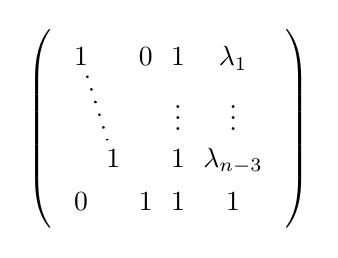
\begin{tikzpicture}[baseline=(current bounding box.center)]
\matrix (m) [matrix of math nodes,nodes in empty cells,right delimiter={)},left delimiter={(} ]{
1  &  & 0  & 1 & \lambda_1  \\
  & & & \vdots & \vdots \\
 & 1  & & 1 & \lambda_{n-3}    \\
0  & & 1 & 1 & 1 \\
} ;
\draw[loosely dotted, thick] (m-1-1)-- (m-3-2);
\end{tikzpicture}\]
Then $(\mathbb{H}/\Delta(a_1, \dots, a_n),(r_1, \dots r_n)) = (\mathbb{P}_\mathbb{C}^1, (\lambda_1, \dots, \lambda_{n-3}, 1, 0, \infty))$ in $\mathfrak{C}$.
\end{theorem}
Neumann also shows that any such matrix $A$ can be put in the form of Theorem \ref{5.2} without changing the equivariant (with respect to the group action given above) isomorphism type of $V_A$, so indeed this completes the classification of Brieskorn $3$-manifolds.

\subsection{Directions for further research}

Brieskorn manifolds are of considerable interest to topologists and geometers alike, owing in part to the fact that they provide many examples of \textit{exotic spheres} (sometimes called \textit{topological spheres}), $n-$manifolds which are homeomorphic but not diffeomorphic to the Euclidean $n$-sphere. This is perhaps why these manifolds are attributed to Brieskorn, who found in 1966 that the Brieskorn manifolds $M_{(2,2,2,2,6k-1)}$ for $k \in 1, \dots, 28$ furnish all smooth structures on the $7$-sphere, or in other words that these Brieskorn manifolds classify all diffeomorphism classes of $S^7$. \cite{brieskorn_1966}

Also of interest are the \textit{Brieskorn homology spheres}, a class of Brieskorn manifolds $V_{(p,q,r)}$ for which $p,q,r$ are relatively prime. These are $3$-spheres with isomorphic homology groups to the usual $3$-sphere, and are in some sense a generalization of the torus knots exhibited in \S 3. An open problem of some interest is the following, conjectured by Gompf in 2013 \cite{gompf_2013}.
\begin{conjecture}
No nontrivial Brieskorn homology sphere admits a psuedoconvex embedding into $\mathbb{C}^2$,
\end{conjecture}
The \textit{pseudoconvexness} condition is not relevant for this writing, apart from the fact that it is a rather strong condition (for example, it is much stronger than smoothness) to impose, especially seeing as (Gompf notes) many Brieskorn homology spheres do not embed even smoothly into $\mathbb{C}^2$. Still, there have been several partial results in the direction of the affirmative answer to this conjecture (see for example \cite{mark_tosun_2018} for an account of recent developments). This points to these Brieskorn manifolds being objects of particular interest and, even more, the slightly more general notion of \textit{Seifert-fibered homology spheres} are objects of principal interest in the study of Heegaard Floer homology and more generally in low-dimensional topology (\cite{https://doi.org/10.48550/arxiv.2110.13405}, \cite{https://doi.org/10.48550/arxiv.0909.3975}).

More generally, these Brieskorn manifolds provide the most digestible example of the deep topological insight that can be gained from analyzing singularities of algebraic varieties. In particular, the study of canonical and terminal singularities of projective varieties is of great interest in algebraic geometry and specifically the \textit{minimal model program}, the project to, roughly speaking, classify projective algebraic varieties (\textit{i.e.} irreducible algebraic subsets of $\mathbb{P}^n_\mathbb{C}$) up to birational equivalence. My goal for research this summer, and for my senior thesis, is to begin studying these singularities of projective varieties from a more algebraic viewpoint (in contrast to the topological viewpoint of this paper), and in general to build the foundations for further study in algebraic geometry.


\newpage
\bibliographystyle{plain}
\bibliography{bibliography.bib}

\textit{This paper represents my work in accordance with University Regulations. -Thomas Sachen}

\end{document}
